\chapter{SMT}
\label{ch:smt}

Satisfiability Modulo Theories (SMT) je rozšířením SAT (Satisfiability) problému.
SMT rozšiřuje SAT o takzvané teorie jako například celočíselná aritmetika, reálná čísla, bitové vektory a další.
Jméno je odvozeno od toho, že splnitelnost se zkoumá v rámci (modulo) dané teorie.
SMT se používá v různých oblastech formální verifikace softwaru a automatizovaného dokazování~\cite{SMT}.

SMT řešiče integrují hlavní algoritmus pro řešení SAT problémů a poté knihovnu porporovaných teorií.
Kontrétně SMT řešič Z3, jehož architektura je znázorněna na obrázku~\ref{fig:z3-block-diagram},
používá DPLL(T) algoritmus pro SAT\@.

\begin{figure}[H]
    \centering
    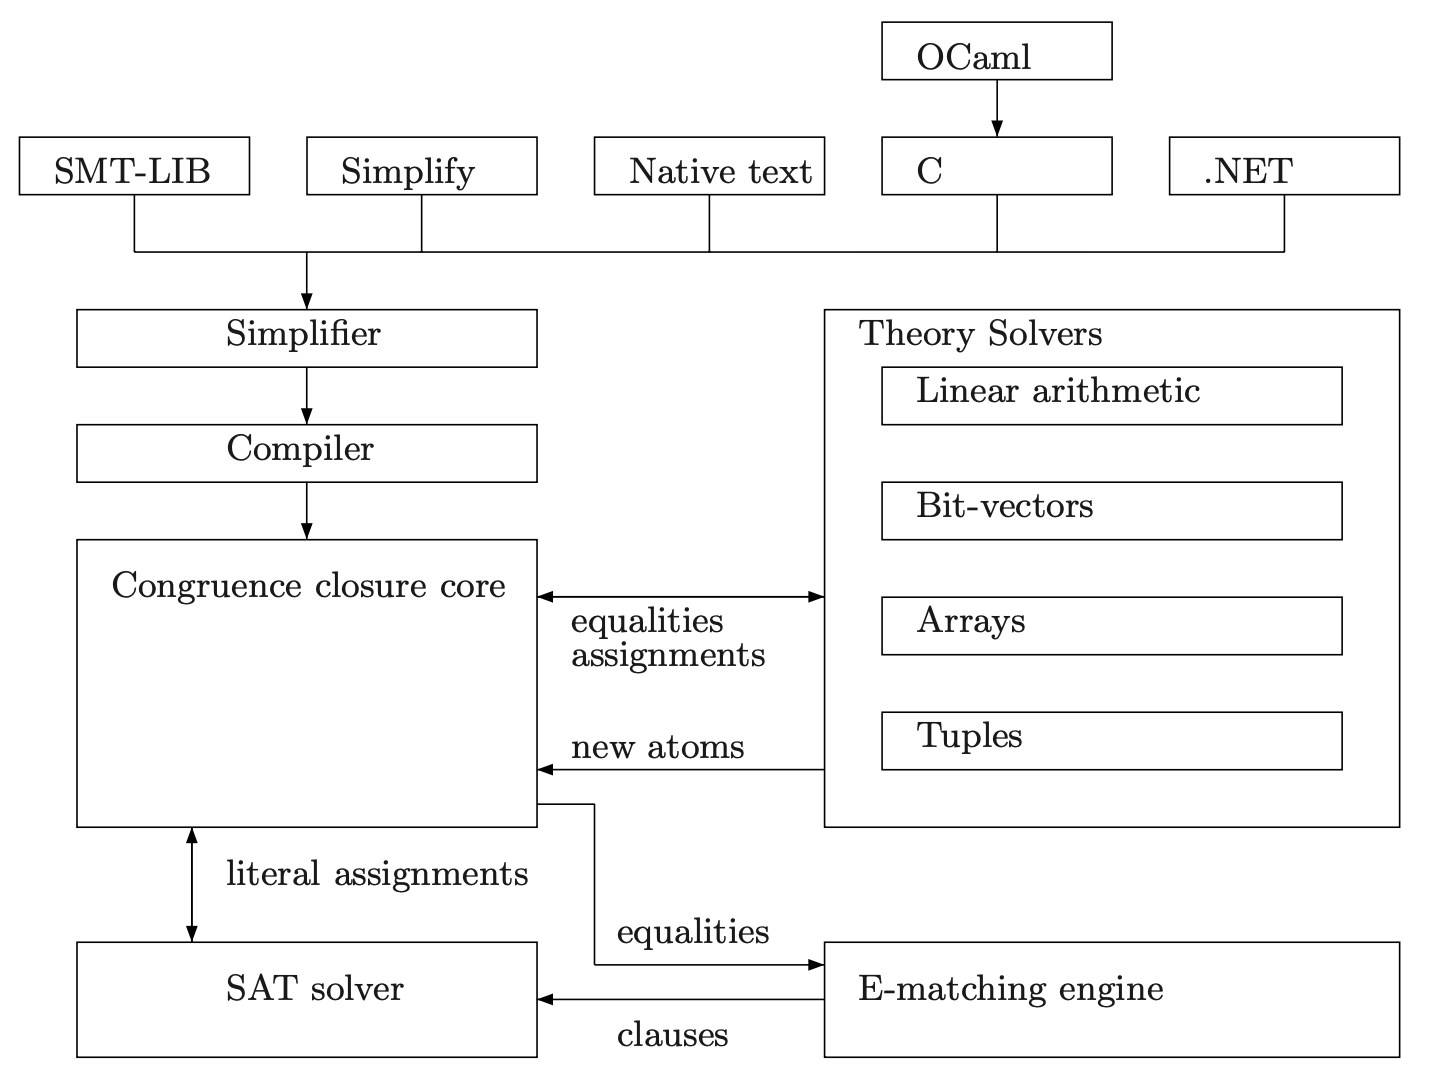
\includegraphics[width=.85\linewidth]{images/smt-structure}
    \caption{
        Blokový diagram SMT řešiče Z3. \\
        Převzato z článku Z3: An Efficient SMT Solver~\cite{Z3}.
    }
    \label{fig:z3-block-diagram}
\end{figure}

Algoritmus DPLL (Davis-Putnam-Logemann-Loveland) představený roku 1961
je algoritmus pro řešení SAT problémů
založený na rekurzivním prohledávání do hloubky, rozhodování o ohodnocení proměnných a zpětné propagaci (backtracking).
Algoritmus je založen na propagaci jednoduchých důsledků (unit propagation) v případě jednoduchých klauzulí
a rozhodování o ohodnocení proměnných v případě složitějších klauzulí.

Rozšířený algoritmus DPLL(T) zahrnuje teorii T, podporovanou SMT řešičem.
Tento algoritmus se skládá ze dvou částí.
První část je algoritmus DPLL pro SAT, který se stará o splnitelnost booleovských proměnných.
SMT řešič kóduje vlastnosti z teorie T do booleovských proměnných a klauzulí.
Druhá část je SMT řešič dané teorie, který dostává kandidátní ohodnocení proměnných od SAT řešiče a kontroluje logickou konzistenci
v rámci dané teorie.
Tento proces se opakovaně provádí a pokud je nalezena neslučitelnost v SMT teorii,
tak SMT řešič informuje SAT řešič o dané neslužitelnosti pomocí konfliktní klauzule.
Tato klauzule je poté přidána do původní formule a DPLL algoritmus pokračuje v hledání dalšího ohodnocení proměnných
v rozšířené formuli~\cite{DPLLT}.




\section{Standard SMT-LIB}
\label{sec:smt-lib}

SMT-LIB je standardizovaný jazyk pro SMT, který definuje syntaxi a sémantiku pro zápis SMT problémů.
Tento standard byl vyvinut pro usnadnění výzkumu, vývoje a porovnávání různých SMT řešičů.
Ukázka~\ref{lst:smt-lib-example} ukazuje příklad SMT-LIB kódu pro booleovskou formuli

\begin{equation*}
    p \land (p \lor \neg q)
\end{equation*}
kde $p$ a $q$ jsou booleovské proměnné.

\begin{listing}[H]
    \begin{minted}{lisp}
    (set-logic QF_UF)

    (declare-const p Bool)
    (declare-const q Bool)

    (assert (and p (or p (not q))))

    (check-sat)
    (get-model)
    \end{minted}
    \caption{Příklad SMT-LIB kódu pro booleovskou logiku}
    \label{lst:smt-lib-example}
\end{listing}

Pomocí volání funkce \texttt{check-sat} lze zjistit, zdali existuje řešení pro danou formuli.
Pokud ano, SMT-LIB vrátí \texttt{sat}, jinak vrátí \texttt{unsat}.
Pokud je výsledek \texttt{sat}, lze pomocí funkce \texttt{get-model} získat konkrétní hodnoty proměnných, které splňují danou formuli.
Pro tuto formuli byl nalezen model s ohodnocením $p = \texttt{true}$ a $q = \texttt{false}$.
Zvolená logika je \texttt{QF\_UF} (Quantifier-Free Uninterpreted Functions),
což znamená, že se jedná o logiku bez kvantifikátorů nad neinterpretovanými funkcemi.
Neinterpretované funkce jsou funkce, které nemají žádnou konkrétní interpretaci a jejich význam je dán pouze jejich syntaktickým zápisem.
Konstanty reprezentující proměnné jsou deklarovány pomocí funkce \texttt{declare-const},
což je pouze syntaktický cukr pro neinterpretovanou funkci bez parametrů~\cite{SMTLIB}.

Ukázka~\ref{lst:smt-lib-example-int} zobrazuje příklad SMT-LIB kódu pro celočíselnou aritmetiku.
Konkrétně se jedná o příklad se soustavou dvou rovnic o dvou neznámých.

\begin{align*}
    x + y &= 5 \\
    2x − y &= 4
\end{align*}
kde $x$ a $y$ jsou celočíselné proměnné.

\begin{listing}[H]
    \begin{minted}{lisp}
    (set-logic QF_LIA)

    (declare-const x Int)
    ; syntax sugar for (declare-fun y () Int)
    (declare-const y Int)

    (assert (= (+ x y) 5))
    (assert (= (- (* 2 x) y) 4))

    (check-sat)
    (get-model)
    \end{minted}
    \caption{Příklad SMT-LIB kódu pro celočíselnou aritmetiku}
    \label{lst:smt-lib-example-int}
\end{listing}

Pomocí SMT řešiče lze získat řešení $x = 3$ a $y = 2$.

Pokud bychom měli funkci, která by mohla obsahovat více než jedno řešení,
jako například

\begin{equation*}
    x^2 - 4 = 0
\end{equation*}
mohli bychom interaktivně s SMT řešičem procházet jednotlivá řešení.
Po získání prvního řešení bychom mohli přidat další podmínku, která by vyloučila
první nalezené řešení a pokračovat v hledání dalších řešení.
Tento interaktivní přístup je vhodné naprogramovat, ale výsledné volání SMT řešiče
by vypadalo stejně, jako v následujícím příkladu~\ref{lst:smt-lib-example-sqrt}.

\begin{listing}[H]
    \begin{minted}{lisp}
    (set-logic QF_LIA)

    (declare-const x Int)

    (assert (= (- (* x x) 4) 0))

    (check-sat)
    (get-model)

    (assert (not (= x 2)))

    (check-sat)
    (get-model)

    (assert (not (= x -2)))

    (check-sat)
    \end{minted}
    \caption{Příklad SMT-LIB kódu pro hledání více řešení}
    \label{lst:smt-lib-example-sqrt}
\end{listing}

Tímto postupem nám SMT řešič postupně oznám dvakrát výsledek \texttt{sat} s modelem pro proměnnou $x$ s hodnotou $2$ a $-2$.
Nakonec oznámi výsledek \texttt{unsat}, což znamená, že neexistuje další řešení a program by měl skončit.


% https://smt-lib.org/language.shtml

%\section{Standard SyGuS}
%% https://sygus-org.github.io/language/

\section{SMT řešiče}
\label{sec:smt-resice}

SMT řešiče jsou nástroje pro automatické dokazování splnitelnosti SMT formulí.
Každá řešič podporuje různé teorie, ale většina moderních řešičů podporuje stejný vstupní formát SMT-LIB verze~2.

\subsection{Eager přístup}

\subsection{Lazy přístup}

\subsection{Alt-Ergo}
\label{subsec:alt-ergo}

\subsection{CVC}
\label{subsec:cvc}

\subsection{Z3}
\label{subsec:z3}